\chapter{Framework Himalaya (20 pages) }
	Himalaya est un framework d'édition d'image s'inspirant des frameworks nodaux et de la technique de megatextures. Il fut conçu par moi même avant la
	réalisation de ce mémoire dans le but de créer un logiciel de peinture permettant l'édition non destructive, la composition non linéaire, et d'être
	compatible avec la technique de mégatexture afin de pouvoir être utilisé dans le jeu vidéo. 


	\section{Structures de données}
		\subsection{Les Tiles}
		Comme dans bien d'autres framework, les images d'himalaya sont divisés en grilles de tiles. Un tile est donc un bitmap rectangulaire correspondant
		à une petite région de l'image. Himalaya fait un plus grand usage des tiles que d'autres frameworks puisque toute opération prend des tiles
		en entrée et en sortie. Un tile représente donc la plus petite unité de traitement, et un intérèt particulier doit être apporté à sa conception.

		\subsubsection{Structure du tile}
			Il y a trois caractéristiques importantes à prendre en compte lorsque l'on conçoit un tile:
			\begin{description}
				\item[Sa taille en mémoire]Un premier intérèt des tiles est qu'ils sont une unité de mémoire pouvant être suffisemment petite
				pour tenir intégralement dans les caches du processeur et ainsi éviter des accès cache invalides fort coûteux en temps de calcul.
				Les processeurs de différent modèles ont différentes taille de cache et différentes manières de les gérer. Plus le tile est petit,
				plus il sera rapide de les traiter sur une grande gamme de processeurs.
				
				Cependant, si le tile est trop petit, les gains réalisés par sa taille sont perdu par la surcharge de travail que doit faire le
				framework pour gérer ces tiles. 

				En outre, si tous les tiles ont la même taille en mémoire, on réduit les risques de fragmentation, et on peut faire des
				allocateurs optimisés qui allouent les tiles de manière contigue et réutilisent les tiles libérés.

				\item[Sa taille en pixel] Si tous les pixels ont la même taille en pixel, alors les images de dimensions égales seront
				toujours divisées en tiles de la même manière, ce qui rend plus simples beaucoup d'algorithmes du framework.
				la programmation des opérations en sera également facilitée. 

				Cependant, un framework moderne doit prendre en compte la gestion de modèles colorimétriques, et niveaux de quantification
				différents. La représentation d'un pixel peut donc avoir des empreintes mémoire différentes, il faudra donc choisir entre
				avoir des tiles de même taille pixel, ou des tiles de même taille mémoire.

			\begin{figure}[h]
				\centering
				\subfloat[Un tile normal]{ \label{fig:render} 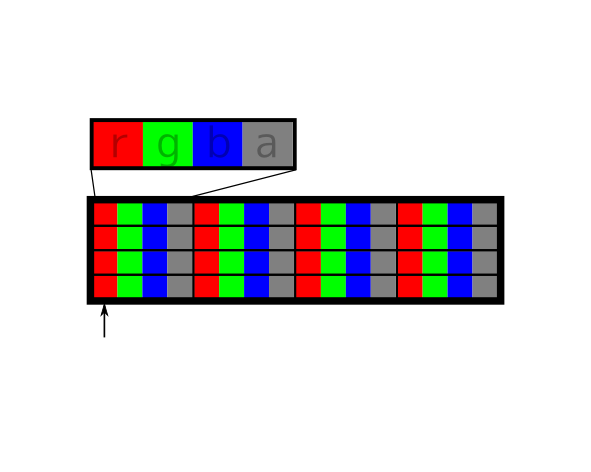
\includegraphics[width=0.5\textwidth]{images/tile-a} }
				\subfloat[Un tile aux canaux séparés]{ \label{fig:render-hsv} 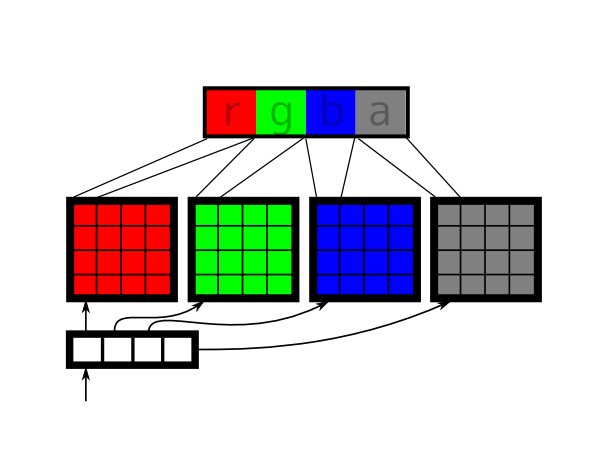
\includegraphics[width=0.5\textwidth]{images/tile-b} }
				\caption{Deux structures de tiles}
				\label{fig:tilestruct}
			\end{figure}
				\item[La répartition des pixels dans le tile] La manière commune de représenter un pixel au sein d'un bitmap est d'avoir
				toutes ses composantes placées dans des emplacement contigus. Une autre manière est de placer chaque composante dans un
				bitmap séparé. Un tile étant alors constitué de plusieurs bitmaps. L'intéret de cette technique est que les tiles de même
				quantisation ont la même taille en pixel, et les bitmaps les constituant la même taille en mémoire. Un autre intérèt est
				qu'il est maintenant beaucoup plus facile de programmer des opérations qui peuvent gérer un nombre quelconque de composantes
				par pixel.

				Cependant, cela implique que l'accès à un pixel nécessite autant d'accès mémoires que de composantes, ce qui ralentit 
				l'exécution du programme. 
			\end{description}

		\subsubsection{Comparaison des tiles}
			Le tableau TODO représente le résultat d'expériences qui résument les concepts précedemment exposés. Dans ce tableau, deux opérations
			sont testées : \emph{colorfill} consiste à remplir une image de $8192^2$ pixels \emph{RGBA} 8bits/composante d'une couleur unie. \emph{blend} consiste 
			en fusionner deux images de $8192^2$ pixels \emph{RGBA} 8 bits/composante par opacité. Ces deux opérations 
			sont utilisées très couramment pour la réalisation de peintures. 

			Ces opérations sont appliquées selon des schémas différents: \emph{colorfill\_full} remplit tous les tiles de l'image, alors que \emph{colorfill\_single}
			remplit un tile choisit au hasard autant de fois qu'il y a de tiles dans l'image. Le même nombre de pixels est donc traité dans les deux tests,
			mais le second devra accéder régulièrement à de nouvelles zones mémoire.

			Même chose pour les operations \emph{blend} : \emph{blend\_full} fusionne les tiles des deux images, \emph{blend\_single} fusionne deux tiles
			sélectionnés au hasard, \emph{blend\_intermediate} fusionne toute l'image sur un seul tile. Ce dernier test est fort représentatif de la
			manière dont les tiles sont utilisés dans Himalaya.

			Ensuite les tiles normales sont comparées aux tiles à canaux séparés. 
			

			\begin{table*}
				\label{tileperf}
				\tiny
				\begin{tabular*}{\textwidth}{@{\extracolsep{\fill}} | r | c || c | c | c | c | c | c | c | c | c |}
					\hline
					\multicolumn{2}{|r||}{Largeur des tiles}& 8	& 16	& 32	& 64	& 128	& 256	& 512	& 1024	& 2048	\\
					\hline 
					Test	& Tile &\multicolumn{9}{ c|}{Temps de calcul moyen sur 5 expériences (secondes)}\\
					\hline
					\emph{colorfill\_single} & Normal 	& 0.78	& 0.64 	& 0.58	& 0.57	& 0.49	& 0.28	& 0.28	& 0.28	& 0.31	\\
					\emph{colorfill\_full} & Normal 	& 1.14	& 0.7 	& 0.65	& 0.63	& 0.55	& 0.44	& 0.47	& 0.44	& 0.51	\\
					\emph{colorfill\_single}& Séparé 	& 1.30	& 1.06 	& 1.04	& 1.06	& 0.97	& 0.79	& 0.79	& 0.79	& 0.80	\\
					\emph{colorfill\_full} & Séparé 	& 2.14	& 1.39 	& 1.16	& 1.12	& 1.10	& 1.03	& 1.00	& 1.01 & 1.01	\\
					\hline\hline
					\emph{blend\_single} & Normal 		& -	& 3.12 	& 2.98	& 3.0	& 3.08	& 4.16	& 13.58	& 19.97	& 22.60	\\
					\emph{blend\_inter} & Normal 		& -	& 5.31 	& 5.20	& 4.96	& 5.12	& 4.85	& 13.49	& 20.46	& 20.64	\\
					\emph{blend\_full} & Normal 		& -	& 5.39 	& 5.19	& 5.17	& 5.0	& 5.42	& 13.15	& 20.44	& 21.12	\\
					\emph{blend\_single}& Séparé		& -	& 6.29 	& 5.64	& 5.39	& 6.61	& 6.50	& 18.67	& 27.48	& 28.92	\\
					\emph{blend\_inter}& Séparé		& -	& 6.55 	& 5.69	& 5.50	& 6.55	& 6.74	& 20.22	& 27.77	& 27.48	\\
					\emph{blend\_full} & Séparé	 	& -	& 6.68 	& 5.82	& 5.45	& 6.59	& 6.78	& 18.39	& 27.41 & 27.23	\\
					\hline
				\end{tabular*}
			\end{table*}
			\begin{figure}[h]
				\centering
				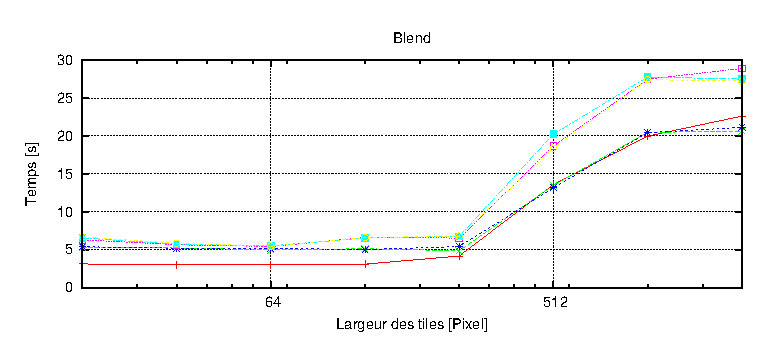
\includegraphics[width=\textwidth]{images/tilegraph.eps} 
				\label{fig:tilegraph}
			\end{figure}
		\subsubsection{Analyse des performances}
			On peut tirer plusieurs conclusion de ces expériences:
			\begin{itemize}
				\item Les tiles doivent être les plus grands possibles, pour diminuer le 
			nombre d'appels de fonctions, mais ne doivent pas être trop grands, sinon les performances sont très fortement dégradées. 
				\item Les tiles à canaux séparés sont jusque 2 fois plus lents que les tiles normaux.
				\item Le schémà d'accès aux tiles en mémoire a un impact non négligable mais plus marqué sur les tiles normaux.
				\item Le temps pour faire la fusion d'un même nombre de pixels peut différer de 970\% selon le type de tile, sa taille et la
				manière dont il est utilisé, puisque cette opération représente la grande majorité du temps de calcul du framework, ce choix
				est particulièrement important.
			\end{itemize}
			Enfin, il ne faut pas oublier que ces expériences ommettent deux facteurs importants: Le fait que la gestion des tiles dans le framework 
			est bien plus lourde, ce qui favorise les tiles plus grands, et le fait que les tiles plus petits permettent plus de précision dans 
			la localisation des opérations, ce qui permet de réduire le nombre de pixels accédés à chaque opération.

			Déterminer l'importance de ces deux facteurs requiert d'avoir des données d'utilisation du framework représentatives, par exemple
			avec des tests utilisateur. 
		\subsubsection{Structure finale}
			Le choix s'est porté sur des tiles normaux de taille fixe de $32\times32$ pixels, et ce quelque soit le modèle colorimétrique utilisé.
		\subsection{Les Frames}
			La Frame est la structure de donnée qui organise les tiles. Elle a deux utilités: Représenter une image bitmap et servir de cache aux
			résultats des opérations. La Frame est en fait une pyramide de tiles creuse, implémentée par des Quad-Trees.
			\subsubsection{Les Quad-Trees}
				Les Quad-Trees sont composés de FrameNodes. Ceux-ci sont une référence optionelle vers un tile, et quatre références, optionelles,
				vers des noeuds enfants. La tile référencée par le noeud représentant les quatres tiles des noeuds enfants à une échelle deux
				fois plus petite.

				Chaque ensemble de noeuds de la même profondeur représente ainsi un bitmap à l'échelle deux fois plus petite que l'ensemble de
				noeuds à la profondeur suivante.

			\subsubsection{Placer une image dans le Quad-Tree}
				Afin d'éviter d'avoir des Quad-Trees inutilement profond, les images sont stoquées au niveau le moins profond pouvant les contenir,
				soit $ceil( \log_2( max(size_x,size_y)/32))$, $size_x$,$size_y$ représentant la largeur et la hauteur de l'image en pixels.
				Cette profondeur est ensuite stoquée dans la Frame afin de pouvoir identifier le niveau de résolution native.

			\subsubsection{Référencer les Tiles dans le Quad-Tree}
				Les tiles sont référencés par trois coordonnées $(t_x,t_y,t_z)$. $t_x,t_y$ représente les coordonnées spatiales du tile, $t_x$ valant
				zéro à l'extrémité gauche du bitmap, et étant positif à droite. $t_y$ vaut zéro à l'extrémité supérieure du bitmap et est positif vers le bas,
				et ce quelque soit l'échelle représentée.
				
				$t_z$ représente le niveau d'échelle. Il vaut $0$ au niveau le plus profond, correspondant à la résolution native, et est positif
				pour les échelles inférieures. En effet, si l'on aggrandit ou réduit l'image, on modifie la profondeur du quad-tree, et donc la profondeur à 
				laquelle se trouve la résolution native. Cette définition du $t_z$ permet donc de référencer les tiles de l'image indépendemment de leur taille.
				
				Sa valeur maximale dépend donc de la taille de l'image stockée
				dans la Frame. Cependant, comme nous voulons pouvoir indexer les pixels indépendemment, la largeur de l'image ne peut dépasser
				\emph{MAX\_INT}, Ce qui correspond à une valeur maximale de $t_z$ de $26$ sur les architectures 32bits, avec des tiles de 32 pixels
				de coté.
				
			\subsubsection{Les coordonnées négatives}
				Lorsque la Frame sert à stocker un bitmap chargé depuis le disque, les pixels le constituant, et donc les tiles, sont toujours
				à des coordonnées positives. Cependant, il est pratique de pouvoir également stocker des pixels de coordonnées négatives, afin
				de disposer du plan complet pour pouvoir stocker le résultat de transformations géométriques. Pour ce faire, la Frame
				stoque un Quad-Tree par quadrant, et les tiles aux coordonnées négatives sont redirigées vers les Quad-Tree correspondant.

			\subsubsection{Le Tile de fond}
				Lorsque la frame est utilisée pour contenir un bitmap, celle-ci dispose d'un Tile de fond. Celui-ci n'est pas repris
				dans les Quad-Tree et est d'une couleur unie correspondant au 'fond' de l'image, habituellement une couleur transparente.
				Lorsque l'on tente d'accéder à une coordonnée qui ne correspond à aucun noeud des Quad-Trees, ce que l'on a atteint une zone
				correspondant au fond de l'image, et le tile de fond est renvoyé. Ceci permet de réduire l'espace pris par des zones vides
				de l'image.

		\subsection{Image}
		\subsection{Opérations}
		\subsection{États}
	\section{Algorithmes}
		\subsection{Rasterisation}
		\subsection{Dessin}
		\subsection{Sauvegarder l'état}
		\subsection{Charger un état}
		\subsection{Supprimer un état}
		\subsection{Modifier une opération}
	\section{Gestion de la cache}
	\section{Utilisation}
		\subsection{API publique}
		\subsection{Undo / Redo}
		\subsection{Modèle objet par calques}
		\subsection{Modèle objet nodal}
		\subsection{Traits de pinceau}

\chapter{Localité des operations (20 pages)}
	\section{Opérations vectorisées}
		\subsection{Impact sur l'API}
		\subsection{Évaluation des performances}
	\section{Bounding Boxes}
		\subsection{Algorithme Inline}
		\subsection{Algorithme Off-line}
		\subsection{Multi-Niveaux}
		\subsection{Impact sur l'API}
		\subsection{Évaluation des performances}

\chapter{Anti-aliasing (15 pages) }
	\section{Primitive de dessin}
	\section{Problèmes d'échelle}
		\subsection{Oversampling}
	\section{Problèmes de superposition}
	\section{Problèmes de bandes}
	\section{Problème de blending à faible opacité}
	\section{Problème de précision de positionement}
\chapter{Test utilisateurs (10 pages) }
	\section{Procédure}
	\section{Résultats}
	\section{Analyse}
\chapter{Comparaison d'Himalaya aux autres frameworks}
\chapter{Conclusion}
